%%
\chapter{Domain modeling and goal definition in EMF and \viatra{}}
%%

In this chapter the creation of initial artifacts is presented: domain models and graph patterns.
Domain modeling is an essential part of our framework, as the domain model defines the structure of the runtime live model, and affects the whole process. 
After the domain model is known, graph pattern can be specified, which will be used later in runtime analysis.
In the framework domain modeling are technologically backed up by EMF (Eclipse Modeling Framework), 
while graph pattern definition and processing are provided by \viatra{}.

\section{Eclipse Modeling Framework}


\begin{figure}[!ht]
	\begin{center}
		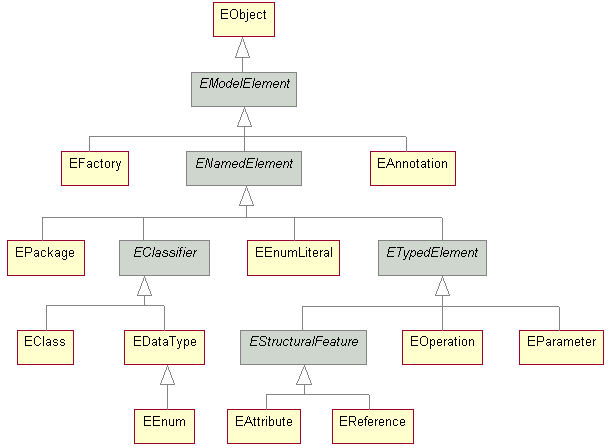
\includegraphics[width=0.5\textwidth]{figures/EcoreHierarchy.png}
		\caption{Hierarchy of Ecore elements}
		\label{fig:ecore-hierarchy}
	\end{center}
\end{figure}

Eclipse Modeling Framework (EMF) is an Eclipse based technology, which provides tools for model based developement: 
Ecore for metamodeling (Ecore actually defines a meta meta-model for metamodeling), and various tools like java code generation from ecore models, etc.

Ecore metamodeling is highly similar to defining class diagrams in UML, however, 
Ecore is more suitable for data and structural modeling: Interfaces are not a part of it, even though it can be substituted by abstract classes.

The hierarchy of Ecore elements can be seen on figure \ref{fig:ecore-hierarchy}, while its structure on \ref{fig:ecore-relations}
EObject is a base for everything, and its main purpuse to define the containment hierarchy of the model. 
EObjects can contain each other in a strict tree structure, circular containments are not permitted.
EModelElement expands EObject by giving the possibility to annotate them.

An Ecore model contains packages (EPackage). 
Packages have a namespace URI (nsURI), which can be used to refer it in other context eg.\ Viatra graph pattern definition.
Packages can contain other subpackages, classes (EClass), enumerations(EEnum), and data types(EDataType).

Classes have structural features: references and attributes (EStructuralFeature, EReference, EAttribute); also they have operations (EOperation).
References and attributes have multiplicity, defining their lower and upper bound is also possible.
ECore also provides tools to define containment hierarchy in the domain model itself: References can be containment or containing reference (considering direction of the reference). 
Two way navigation can be achieved by defining two reference and set them as the EOpposite of each other. A reference cannot be the EOpposite of itself, but its not a problem in most of the cases (eg.: \texttt{Human} class and \texttt{Spuse} reference). 

Multiple inheritance is supported for classes (eSuperTypes refers to direct base classes, and eAllSuperTypes for all transitively inherited base classes).

Besides classes, packages can contain enumerations and data types. 
Basic data types, like EString, EInt, EBoolean etc.\ are defined by EMF, so its mostly never necessary to define others.
Enumerations are consists of EEnumLiterals. 
EEnumLiterals have an integral unique value, and its name is encapsulated in its EEnumerator instance.





\begin{figure}[!ht]
	\begin{center}
		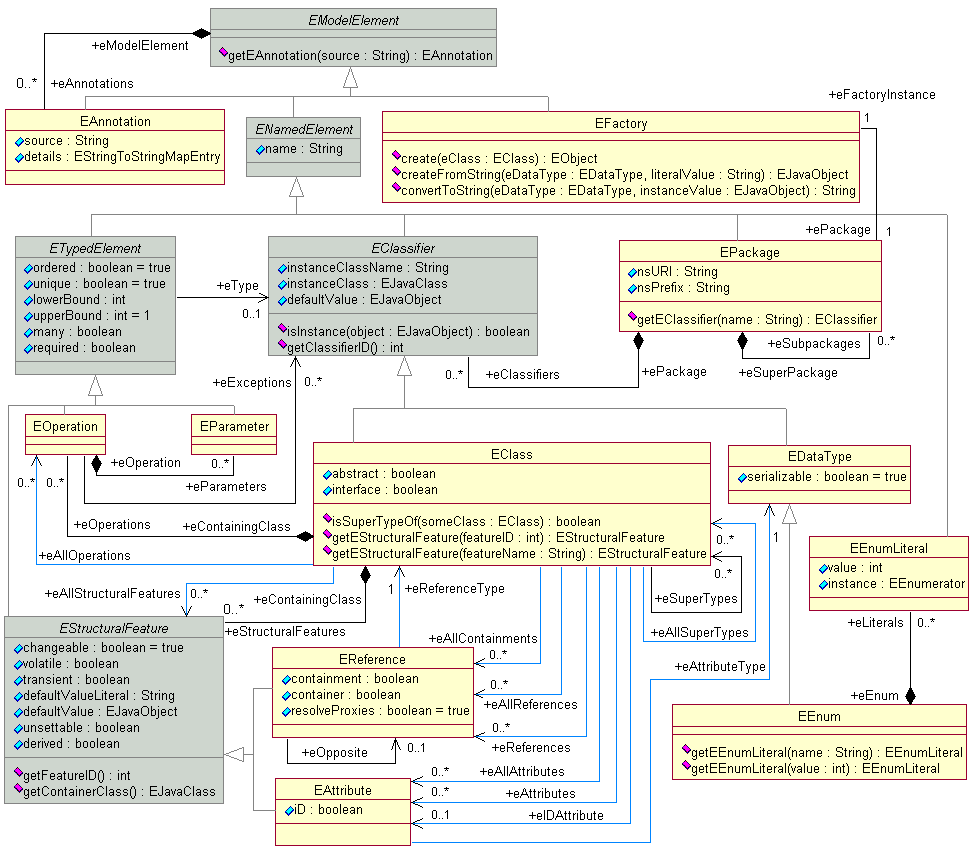
\includegraphics[width=\textwidth]{figures/EcoreRelations.png}
		\caption{Relations between Ecore elements}
		\label{fig:ecore-relations}
	\end{center}
\end{figure}

	

\section{\viatra{} query language (VQL)}

As stated before, graph patterns can be defined using \viatra{} query language (VQL). 
The language syntax is simple, altough complex queries are not always self evident how to be expressed, because graph patterns structure is somewhat strict.

\subsection{Pattern definition}
Patterns and its bodies can be given by the \emph{pattern} keyword. 
Parameters must be specified after the parameter name in round brackets. 
Bodies of the pattern are given in curly brackets, separeted by the \emph{or} keyword

\begin{minipage}{\textwidth}
\begin{lstlisting}[language=vql]
pattern patternName( p1: Type1, p2: Type2){
... // Constraints for first body
} or {
... // Constraints for first body
}
\end{lstlisting}
\end{minipage}


\subsection{Constraints}
Constraints are given like statements. 
Each constraint is followed by a semicolon.

\vspace{\abovedisplayskip}
\begin{minipage}{\textwidth}
Type constraint can be given by specifying the type, then the object in round brackets.
\begin{lstlisting}[language=vql]
pattern patternName( p1 ){
	Type1(p1);
}
\end{lstlisting}
\end{minipage}
\vspace{\belowdisplayskip}

\begin{minipage}{\textwidth}
Reference constraint can be given by specifying which type's which reference must be checked, then giving the source and target variables in round brackets:
\begin{lstlisting}[language=vql]
pattern patternName( p1: Type1, p2: Type2 ){
	Type1.ReferenceLabel(p1, p2);
}
\end{lstlisting}
\end{minipage}
\vspace{\belowdisplayskip}

\begin{minipage}{\textwidth}
Other patterns can be used as constraint with the find keyword:
\begin{lstlisting}[language=vql]
pattern patternName( p1: Type1, p2: Type2, p3: Type3 ){
	find otherPatternName(p1, p2);
	find otherPatternName(p2, p3);
}
\end{lstlisting}
\end{minipage}
\vspace{\belowdisplayskip}

\begin{minipage}{\textwidth}
Negative application condition can be expressed by neg find keyword:
\begin{lstlisting}[language=vql]
pattern patternName( p1: Type1, p2: Type2 ){
	neg find otherPattern(p1, p2);
	Type1.reference(p1, p2);
}
\end{lstlisting}
\vspace{\belowdisplayskip}

Also, we can use underscore if we don't want that the other pattern match occurs with \emph{any} value at the underscores. (neg find can be used to express negated expressions along with negated existential quantification)

\begin{lstlisting}[language=vql]
pattern patternName( p1: Type1 ){
neg find otherPattern(p1, _);
}
\end{lstlisting}
\end{minipage}
\vspace{\belowdisplayskip}
